\documentclass[11pt]{article}
\usepackage[a4paper,margin=1in]{geometry}
\usepackage{amsmath,amssymb}
\usepackage[T1]{fontenc}
\usepackage{lmodern}
\usepackage{microtype}
\usepackage{xcolor}
\usepackage{footnote}
\usepackage{tikz}
\usetikzlibrary{arrows.meta,calc}

\setlength{\parindent}{0pt}
\setlength{\parskip}{0.5em}

\newcommand{\promptbox}[1]{%
  \begin{savenotes}%
  \begingroup\setlength{\fboxsep}{10pt}\noindent
  \colorbox{blue!8}{\parbox{\dimexpr\linewidth-2\fboxsep\relax}{\textbf{Prompt. }#1}}
  \endgroup
  \end{savenotes}%
}
\newcommand{\resultbox}[1]{%
  \begin{savenotes}%
  \begingroup\setlength{\fboxsep}{10pt}\noindent
  \colorbox{purple!8}{\parbox{\dimexpr\linewidth-2\fboxsep\relax}{\textbf{Result. }#1}}
  \endgroup
  \end{savenotes}%
}
\newcommand{\examplebox}[1]{%
  \begin{savenotes}%
  \begingroup\setlength{\fboxsep}{10pt}\noindent
  \colorbox{green!8}{\parbox{\dimexpr\linewidth-2\fboxsep\relax}{\textbf{Example. }#1}}
  \endgroup
  \end{savenotes}%
}

\title{\textbf{Book 1 --- Lecture 2 --- Exercise 8}\\[2mm]
\large Velocity, Speed, and Acceleration for Four Plane Motions}
\author{}
\date{}

\begin{document}
\maketitle

\promptbox{Calculate the velocity, speed, and acceleration for each of the
following position vectors. If you have graphing software, plot each position
vector, each velocity vector, and each acceleration vector:
\begin{align*}
\text{(i)}\quad \mathbf{r}(t) &= \bigl(\cos(\omega t),\,e^{\omega t}\bigr),\\
\text{(ii)}\quad \mathbf{r}(t) &= \bigl(\cos(\omega t-\phi),\,\sin(\omega t-\phi)\bigr),\\
\text{(iii)}\quad \mathbf{r}(t) &= \bigl(c\cos^3 t,\,c\sin^3 t\bigr),\\
\text{(iv)}\quad \mathbf{r}(t) &= \bigl(c(t-\sin t),\,c(1-\cos t)\bigr).
\end{align*}
\footnote{Here \(\omega,\phi,c\) are constants and \(t\) is time. The exponential
is \(e^{\omega t}\) (not \(\exp(\omega)\) at a single point). The cycloid uses
\(\cos t\) (a common slip is ``\texttt{cost}'' for \(\cos t\)). Plotting is
optional but helps intuition: \(\mathbf{v}\) is tangent to the path and
\(|\mathbf{v}|\) is the scalar speed.}}

Throughout, \(\mathbf{v}=\dfrac{d\mathbf{r}}{dt}\) and
\(\mathbf{a}=\dfrac{d\mathbf{v}}{dt}\). Speed is \(|\mathbf{v}|\).

\section*{(i)\quad \(\mathbf{r}=\bigl(\cos(\omega t),\,e^{\omega t}\bigr)\)}
Components \(x=\cos(\omega t)\), \(y=e^{\omega t}\). Then
\[
v_x=-\omega\sin(\omega t),\qquad v_y=\omega e^{\omega t},
\qquad
|\mathbf{v}|=|\omega|\sqrt{\sin^2(\omega t)+e^{2\omega t}}.
\]
Also
\[
a_x=-\omega^2\cos(\omega t),\qquad a_y=\omega^2 e^{\omega t}.
\]
The path is \emph{not} a circle; speed grows roughly like \(|\omega|e^{\omega t}\)
for \(\omega t\gg 1\).

\paragraph{Figure (i).}
The sketch uses \(\omega=1\) and plots \(x=\cos t\), \(y=e^{t}\) for \(t\in[-0.5,1.1]\)
(the vertical scale is compressed so the curve fits on the page).

\begin{center}
\begin{tikzpicture}[>=Latex, thick, trig format=rad, x=1.65cm, y=0.38cm]
  \draw[->] (-1.15,0) -- (1.2,0) node[below=2pt, font=\small]{$x$};
  \draw[->] (0,-0.35) -- (0,9.2) node[left=2pt, font=\small]{$y$};
  \draw[blue!70!black, line width=0.55pt, domain=-0.5:1.1, samples=72, smooth, variable=\t]
    plot ({cos(\t)},{exp(\t)});
  \pgfmathsetmacro{\ts}{0.45}
  \pgfmathsetmacro{\xc}{cos(\ts)}
  \pgfmathsetmacro{\yc}{exp(\ts)}
  \pgfmathsetmacro{\vx}{-sin(\ts)}
  \pgfmathsetmacro{\vy}{exp(\ts)}
  \coordinate (P) at (\xc,\yc);
  \fill (P) circle (1.6pt);
  \draw[orange!85!black,->, line width=0.5pt]
    ($ (P) + (-0.12*\vx,-0.12*\vy) $) -- ($ (P) + (0.38*\vx,0.38*\vy) $)
    node[right, font=\scriptsize, inner sep=1pt]{$\mathbf{v}$};
\end{tikzpicture}\\[0.35em]
{\small Tangent \(\mathbf{v}\) at a sample time; \(\mathbf{a}\) points up--right here and is not drawn to scale with \(\mathbf{v}\).}
\end{center}

\section*{(ii)\quad \(\mathbf{r}=\bigl(\cos(\omega t-\phi),\,\sin(\omega t-\phi)\bigr)\)}
Let \(\theta=\omega t-\phi\). Then \(x=\cos\theta\), \(y=\sin\theta\), and
\(\dot\theta=\omega\). By the chain rule,
\[
v_x=-\omega\sin\theta,\qquad v_y=\omega\cos\theta,
\qquad
|\mathbf{v}|=|\omega|\sqrt{\sin^2\theta+\cos^2\theta}=|\omega|.
\]
Differentiate again:
\[
a_x=-\omega^2\cos\theta,\qquad a_y=-\omega^2\sin\theta=-\omega^2\,\mathbf{r}.
\]
Uniform circular motion: constant speed \(|\omega|\) and centripetal acceleration
of magnitude \(\omega^2 R\) with \(R=1\) here.

\paragraph{Figure (ii).}
Unit circle with \(\mathbf{r}\) outward, \(\mathbf{v}\) tangent, and \(\mathbf{a}=-\omega^2\mathbf{r}\)
inward (illustration uses \(\omega=1\) for arrow lengths).

\begin{center}
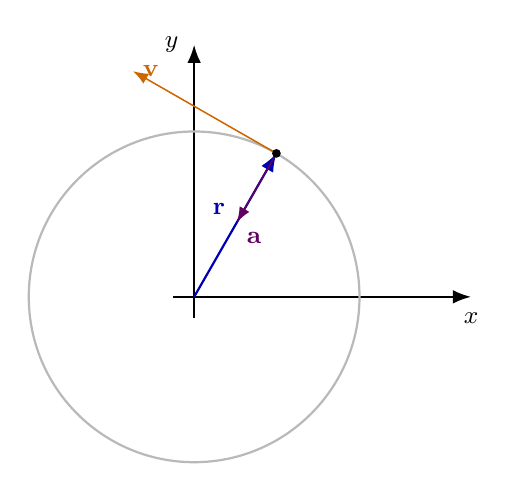
\begin{tikzpicture}[>=Latex, thick, scale=1.05, trig format=rad]
  \def\R{2.0}
  \def\ang{1.05}
  \coordinate (O) at (0,0);
  \coordinate (P) at ({\R*cos(\ang)},{\R*sin(\ang)});
  \draw[->] (-0.25,0) -- (\R+1.35,0) node[below=2pt, font=\small]{$x$};
  \draw[->] (0,-0.25) -- (0,\R+1.05) node[left=2pt, font=\small]{$y$};
  \draw[gray!55] (O) circle (\R);
  \draw[blue!70!black,->] (O) -- (P) node[midway, above left, font=\small]{$\mathbf{r}$};
  \draw[orange!80!black,->, line width=0.55pt] (P) -- ($ (P) + ({-\R*sin(\ang)},{\R*cos(\ang)}) $)
    node[right, font=\small]{$\mathbf{v}$};
  \draw[violet!75!black,->, line width=0.55pt] (P) -- ($ (P) + ({-0.48*\R*cos(\ang)},{-0.48*\R*sin(\ang)}) $)
    node[below right, font=\small]{$\mathbf{a}$};
  \fill (P) circle (1.5pt);
\end{tikzpicture}
\end{center}

\section*{(iii)\quad \(\mathbf{r}=\bigl(c\cos^3 t,\,c\sin^3 t\bigr)\) (astroid / hypocycloid track)}
Write \(x=c\cos^3 t\), \(y=c\sin^3 t\). Then
\[
v_x=-3c\cos^2 t\sin t,\qquad v_y=3c\sin^2 t\cos t.
\]
Factor:
\[
v_x^2+v_y^2
=9c^2\cos^2 t\sin^2 t\bigl(\cos^2 t+\sin^2 t\bigr)
=9c^2\cos^2 t\sin^2 t
=\frac{9c^2}{4}\sin^2(2t),
\]
so
\[
|\mathbf{v}|=\frac{3|c|}{2}\,|\sin(2t)|.
\]
Differentiate \(v_x\) and \(v_y\) (product rule):
\begin{align*}
a_x &= -3c\bigl(-2\cos t\sin^2 t+\cos^3 t\bigr)
=3c\cos t\bigl(2\sin^2 t-\cos^2 t\bigr),\\
a_y &= 3c\sin t\bigl(2\cos^2 t-\sin^2 t\bigr).
\end{align*}
At multiples of \(t=0,\pi/2,\ldots\), the velocity vanishes (cusps of the projected
curve in the plane).

\paragraph{Figure (iii).}
Trace with \(c=1\): \(\bigl(\cos^3 t,\,\sin^3 t\bigr)\) for \(0\le t\le 2\pi\) (four symmetric cusps).

\begin{center}
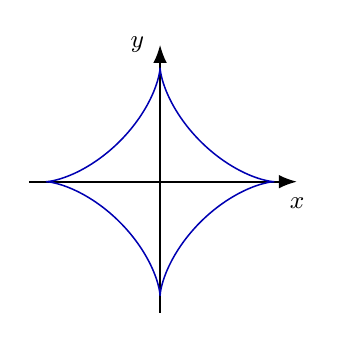
\begin{tikzpicture}[>=Latex, thick, trig format=rad, x=1.45cm, y=1.45cm]
  \draw[->] (-1.15,0) -- (1.2,0) node[below=2pt, font=\small]{$x$};
  \draw[->] (0,-1.15) -- (0,1.2) node[left=2pt, font=\small]{$y$};
  \draw[blue!70!black, line width=0.55pt, domain=0:6.285, samples=140, smooth, variable=\t]
    plot ({pow(cos(\t),3)},{pow(sin(\t),3)});
\end{tikzpicture}
\end{center}

\section*{(iv)\quad Cycloid \(\mathbf{r}=\bigl(c(t-\sin t),\,c(1-\cos t)\bigr)\)}
\[
v_x=c(1-\cos t),\qquad v_y=c\sin t.
\]
Now
\begin{align*}
v_x^2+v_y^2
&=c^2\bigl[(1-\cos t)^2+\sin^2 t\bigr]
=c^2\bigl[1-2\cos t+\cos^2 t+\sin^2 t\bigr]\\
&=2c^2(1-\cos t)=4c^2\sin^2(t/2),
\end{align*}
using \(1-\cos t=2\sin^2(t/2)\). Hence
\[
|\mathbf{v}|=2|c|\,|\sin(t/2)|.
\]
Finally,
\[
a_x=c\sin t,\qquad a_y=c\cos t.
\]

\paragraph{Figure (iv).}
One arch of the standard cycloid with \(c=1\): \(\bigl(t-\sin t,\,1-\cos t\bigr)\) for
\(0\le t\le 2\pi\).

\begin{center}
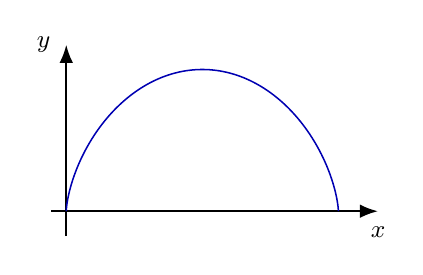
\begin{tikzpicture}[>=Latex, thick, trig format=rad, x=0.55cm, y=0.9cm]
  \draw[->] (-0.35,0) -- (7.2,0) node[below=2pt, font=\small]{$x$};
  \draw[->] (0,-0.35) -- (0,2.35) node[left=2pt, font=\small]{$y$};
  \draw[blue!70!black, line width=0.55pt, domain=0:6.285, samples=120, smooth, variable=\t]
    plot ({\t - sin(\t)},{1 - cos(\t)});
\end{tikzpicture}
\end{center}

\resultbox{\textbf{(i)} \(\mathbf{v}=(-\omega\sin\omega t,\,\omega e^{\omega t})\),
\(|\mathbf{v}|=|\omega|\sqrt{\sin^2\omega t+e^{2\omega t}}\),
\(\mathbf{a}=(-\omega^2\cos\omega t,\,\omega^2 e^{\omega t})\).
\ \textbf{(ii)} \(\mathbf{v}=(-\omega\sin(\omega t-\phi),\,\omega\cos(\omega t-\phi))\),
\(|\mathbf{v}|=|\omega|\), \(\mathbf{a}=-\omega^2\mathbf{r}\).
\ \textbf{(iii)} \(\mathbf{v}=\bigl(-3c\cos^2 t\sin t,\,3c\sin^2 t\cos t\bigr)\),
\(|\mathbf{v}|=\dfrac{3|c|}{2}|\sin 2t|\), \(\mathbf{a}\) as in the section above.
\ \textbf{(iv)} \(\mathbf{v}=c(1-\cos t,\sin t)\), \(|\mathbf{v}|=2|c\sin(t/2)|\),
\(\mathbf{a}=c(\sin t,\cos t)\).}

\examplebox{Graphing: plot \(\mathbf{r}(t)\) as a parametric curve; attach arrows for
\(\mathbf{v}(t)\) and \(\mathbf{a}(t)\) at a few sample times (e.g.\ Desmos,
GeoGebra, Matplotlib, or a CAS). For (ii) the hodograph of \(\mathbf{v}\) is a
circle; for (iv) the rolling-wheel interpretation matches the cycloid form.}

\end{document}
